\chapter{Common Random Variables}\label{S:CommonRVs}

%\remove{
For a continuous RV $X$ with a closed-form expression for the inverse DF $F^{[-1]}$, we can employ \hyperref[A:InvS]{Algorithm~\ref*{A:InvS}} to draw samples from $X$.  \hyperref[T:ContinRVsInvS]{Table~\ref*{T:ContinRVsInvS}}  summarises some random variables that are amenable to \hyperref[A:InvS]{Algorithm~\ref*{A:InvS}}.

\begin{table}[htpb]
\begin{center}
\caption{Some continuous RVs that can be simulated from using \hyperref[A:InvS]{Algorithm~\ref*{A:InvS}}. \label{T:ContinRVsInvS}}
\begin{tabular}{| c | c | c | c |}
\hline
Random Variable $X$ & $F(x)$ & $X=F^{[-1]}(U), \quad U \sim \uniform(0,1)$ & Simplified form \\ \hline
$\uniform(a,b)$ &
\eqref{E:Uniformabcdf} & $a+(b-a)U$ & -- \\
$\exponential(\lambda)$ & \eqref{E:Exponentialpdfcdf} & $\frac{-1}{\lambda} \log(1-U)$ &  $\frac{-1}{\lambda} \log(U)$ \\
$\laplace(\lambda)$ & \eqref{E:LaplaceInvcdf} & $- \frac{1}{\lambda} \ \sign\left( U-\frac{1}{2}\right) \log \left(1 - 2 \left| U-\frac{1}{2} \right| \right)$ & -- \\
$\cauchy$ & \eqref{E:StandardCauchycdf} & $\tan \left(\pi \left(U- \frac{1}{2} \right) \right)$ & $\tan \left(\pi U \right)$ \\
\hline
\end{tabular}
\end{center}
\end{table}
%}%end remove

Next, we familiarise ourselves with the Gaussian or $\normal$ RV.
\begin{model}[$\normal(\mu,\sigma^2)$]
$X$ has a $\normal(\mu,\sigma^2)$ or $\gaussian(\mu,\sigma^2)$ distribution with the location parameter $\mu \in \Rz$ and the scale or variance parameter $\sigma^2 > 0$, if:
\begin{equation}\label{E:Normalpdf}
f(x; \mu, \sigma^2) = \frac{1}{\sigma \sqrt{2 \pi}}
 \exp{\left( - \frac{1}{2 \sigma^2} (x-\mu)^2 \right)}, \qquad x \in \Rz
\end{equation}
$\normal(0,1)$ distributed RV, which plays a fundamental role in asymptotic statistics, is conventionally denoted by $Z$.  $Z$ is said to have the {\bf Standard Normal} distribution with PDF $f(z; 0,1)$ and DF $F(z;0,1)$ conventionally denoted by $\phi(z)$ and $\Phi(z)$, respectively.

There is no closed form expression for $\Phi(z)$ or $F(x;\mu,\sigma)$.  The latter is simply defined as:
\[
F(x;\mu,\sigma^2) = \int_{-\infty}^x f(y;\mu,\sigma)\,dy
\]
We can express $F(x;\mu,\sigma^2)$ in terms of the error function ($\erf$) as follows:
\begin{equation}\label{E:DFNormalviaErf}
F(x;\mu,\sigma^2) = \frac{1}{2} \ \erf \left(  \frac{x-\mu}{\sqrt{2 \sigma^2}} \right)+ \frac{1}{2}
\end{equation}
\end{model}
We 
%\remove{
implement the PDF \eqref{E:Normalpdf} and DF \eqref{E:DFNormalviaErf} for a $\normal(\mu,\sigma^2)$ RV $X$ as \Matlab functions {\tt NormalPdf} and {\tt NormalCdf}, respectively, in \hyperref[Mf: NormalCdfPdf]{Labwork \ref*{Mf: NormalCdfPdf}},  and then 
%}%end remove
produce plots for various $\normal(\mu,\sigma^2)$ RVs, shown in \hyperref[F:plotPdfCdfNormals]{Figure \ref*{F:plotPdfCdfNormals}}.  Observe the concentration of probability mass, in terms of the PDF and DF plots, about the location parameter $\mu$ as the variance parameter $\sigma^2$ decreases.
\begin{figure}[htpb]
\caption{Density and distribution function of several $\normal(\mu,\sigma^2)$ RVs.\label{F:plotPdfCdfNormals}}
\centering   \makebox{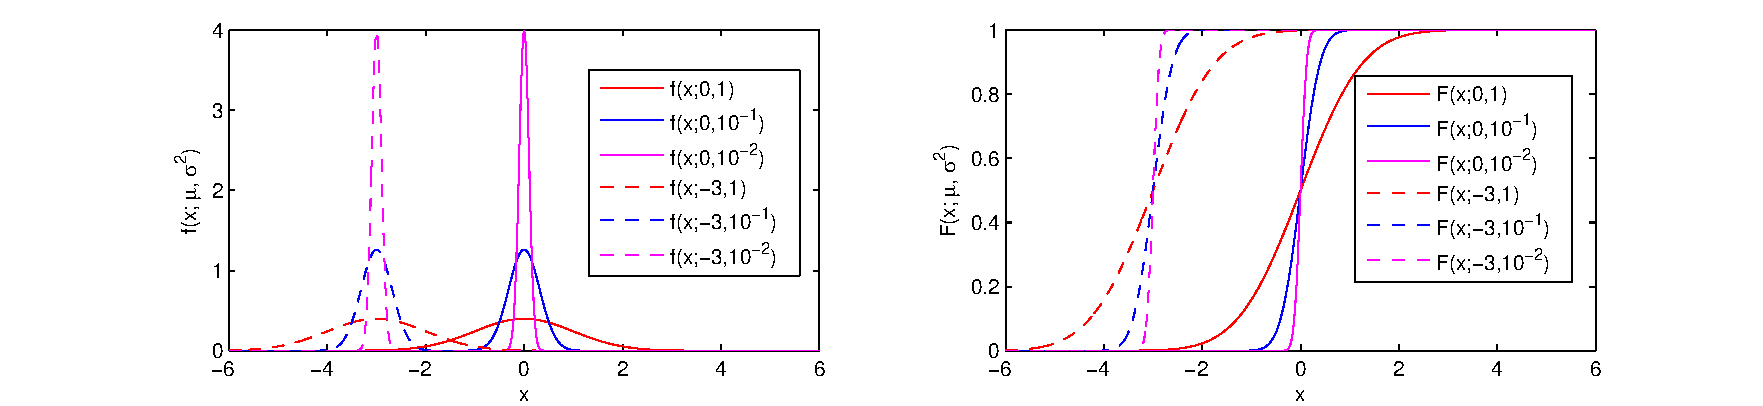
\includegraphics[width=6.5in]{figures/plotPdfCdfNormals}}
\end{figure}

% cse snipped
%\remove{
\begin{labwork}[Compute the  the $\p(X \in (a,b))$ for the $\normal(0,1)$ RV $X$]\label{LW:NormalIntervalProb}
Write a function to evaluate the $\p(X \in (a,b))$ for the $\normal(0,1)$ RV $X$ for user-specified values of $a$ and $b$. [Hint: one option is by making two calls to {\tt NormalCdf} and doing one arithmetic operation.]
\end{labwork}

Simulations \ref*{SIM:Uniformab} and \ref*{SIM:Exponential}, \ref*{SIM:Laplace} and \ref*{SIM:StdCauchy}
produce samples from a continuous RV $X$ with a closed-form expression for the inverse DF $F^{[-1]}$ via \hyperref[A:InvS]{Algorithm~\ref*{A:InvS}} (\hyperref[T:ContinRVsInvS]{Table~\ref*{T:ContinRVsInvS}}).  But only a few RVs have an explicit $F^{[-1]}$.  For example, $\normal(0,1)$ RV does not have an explicit $F^{[-1]}$.
\hyperref[A:InvSbyNumSol]{Algorithm~\ref*{A:InvSbyNumSol}} is a more general but inexact method that relies on an approximate numerical solution of $x$, for a given $u$, that satisfies the equation $F(x)=u$.

\begin{algorithm}
\caption{Inversion Sampler by Numerical Solution of $F(X)=U$ via Newton-Raphson Method}
\label{A:InvSbyNumSol}
\begin{algorithmic}[1]
\STATE {{\it input:} $F(x)$, the DF of the target RV $X$}
\STATE {{\it input:} $f(x)$, the density of $X$}
%\STATE {{\it input:} The fundamental sampler}
\STATE {{\it input:} A reasonable {\tt Stopping Rule}, \\e.g.~a specified tolerance $\epsilon >0$ and a maximum number of iterations {\tt MAX}}
\STATE {{\it input:} a careful mechanism to specify $x_0$}
%\STATE {\it initialise:} set the seed, if any, for the fundamental sampler
\STATE {\it output:} a sample from $X$ distributed according to $F$
\STATE {{\it draw:} $u \sim \uniform(0,1)$}
\STATE{{\it initialise:} $i \gets 0, \qquad x_i \gets x_0, \qquad x_{i+1} \gets x_0 - \frac{F(x_0)-u}{f(x_0)}$}
\WHILE{{\tt Stopping Rule} is not satisfied,\\e.g.~$|F(x_{i})-F(x_{i-1})| > \epsilon$ AND $i < {\tt MAX}$}
\STATE $x_i \gets x_{i+1}$
\STATE $x_{i+1} \gets \left( x_{i} - \frac{F(x_i)-u}{f(x_i)} \right)$
\STATE $i \gets i+1$
\ENDWHILE
\STATE{{\it return:} $x \gets x_i$}
\end{algorithmic}
\end{algorithm}

\begin{simulation}[$\normal(\mu,\sigma^2)$]\label{SIM:NormalByNewRap}
We may employ \hyperref[A:InvSbyNumSol]{Algorithm~\ref*{A:InvSbyNumSol}} to sample from the $Normal(\mu,\sigma^2)$ RV $X$ using the following function.
 \VrbMf[label=Sample1NormalByNewRap.m]{scripts/Sample1NormalByNewRap.m}

We draw five samples from the $\normal(0,1)$ RV $Z$ and store them in $z$ as follows.  The vector $z$ can be obtained by a Newton-Raphson-based numerical transformation of the vector $u$ of $5$ IID samples from the $\uniform(0,1)$ RV.  We simply need to apply the function {\tt Sample1NormalByNewRap} to each element of an array of $\uniform(0,1)$ samples.  \Matlab's {\tt arrayfun} command can be used to apply {\tt @(u)(Sample1NormalByNewRap(u,0,1))} (i.e., {\tt Sample1NormalByNewRap} as a function of $u$) to every element of our array of $\uniform(0,1)$ samples, say {\tt Us}.  Note that $F(z)$ is the same as the drawn $u$ from $U$ at least up to four significant digits.
\begin{VrbM}
>> rand('twister',563987);
>> Us=rand(1,5); % store 5 samples from Uniform(0,1) RV in array Us
>> disp(Us); % display Us
    0.8872    0.2569    0.5275    0.8650    0.8517
>> z=Sample1NormalByNewRap(Us(1),0,1); %transform Us(1) to a Normal(0,1) sample z
>> disp(z); % display z
    1.2119
>> z = arrayfun(@(u)(Sample1NormalByNewRap(u,0,1)),Us); %transform array Us via arrayfun
>> % dislay array z obtained from applying Sample1NormalByNewRap to each element of Us
>> disp(z);
    1.2119   -0.6530    0.0691    1.1031    1.0439
>> % check that numerical inversion of F worked, i.e., is F(z)=u ?
>> disp(NormalCdf(z,0,1));
    0.8872    0.2569    0.5275    0.8650    0.8517
\end{VrbM}
Next we draw five samples from the $\normal(-100.23,0.01)$ RV $X$, store it in an array $x$ and observe that the numerical method is reasonably accurate by the equality of $u$ and $F(x)$.
\begin{VrbM}
>> rand('twister',563987);
>> disp(Us); % display Us
    0.8872    0.2569    0.5275    0.8650    0.8517
>> % transform array Us via arrayfun
>> x = arrayfun(@(u)(Sample1NormalByNewRap(u,-100.23,0.01)),Us);
>> disp(x);
 -100.1088 -100.2953 -100.2231 -100.1197 -100.1256
>> disp(NormalCdf(x,-100.23,0.01));
    0.8872    0.2569    0.5275    0.8650    0.8517
\end{VrbM}
One has to be extremely careful with this approximate simulation algorithm implemented in floating-point arithmetic.  More robust samplers for the $\normal(\mu,\sigma^2)$ RV exist.
However, \hyperref[A:InvSbyNumSol]{Algorithm~\ref*{A:InvSbyNumSol}} is often the only choice when simulating from an arbitrary RV with an unknown closed-form expression for its $F^{[-1]}$.
\end{simulation}
%%% begin of informal CLT excursion
Next, we use our simulation capability to gain an informal and intuitive understanding of one of the most elementary theorems in probability and statistics, namely, the Central Limit Theorem (CLT).  We will see a formal treatment of CLT later.

Informally, the CLT can be stated as follows:\\
``The sample mean of a large number of IID samples, none of which is dominant, tends to the $\normal$ distribution as the number of samples increases.''

\begin{labwork}[Investigating the Central Limit Theorem with IID $\exponential(\lambda=0.1)$ RVs]\label{LW:CLTOfExponentials}
Let us investigate the histograms from $10000$ simulations of the sample mean of $n=10,100,1000$ IID $\exponential(\lambda=0.1)$ RVs as follows:
\begin{VrbM}
>> rand('twister',1973); % initialise the fundamental sampler
>> % a demonstration of Central Limit Theorem (CLT) -- Details of CLT are in the sequel
>> % the sample mean should be a Normal(1/lambda,lambda/n) RV
>> lambda=0.1; Reps=10000; n=10; hist(sum(-1/lambda * log(rand(n,Reps)))/n)
>> lambda=0.1; Reps=10000; n=100; hist(sum(-1/lambda * log(rand(n,Reps)))/n,20)
>> lambda=0.1; Reps=10000; n=1000; hist(sum(-1/lambda * log(rand(n,Reps)))/n,20)
\end{VrbM}
Do you see a pattern in the histograms?

See the histograms generated from the following code that produces sample means from the $\cauchy$ RV:
\begin{VrbM}
>> Reps=10000; n=1000; hist(sum(tan(pi * rand(n,Reps)))/n,20)
>> Reps=10000; n=1000; hist(sum(tan(pi * rand(n,Reps)))/n,20)
>> Reps=10000; n=1000; hist(sum(tan(pi * rand(n,Reps)))/n,20)
\end{VrbM}
\end{labwork}
\begin{classwork}[Why doesn't the sample mean of the $\cauchy$ RV ever settle down?]
Explain in words why the mean of $n$ IID samples from the $\cauchy$ RV ``is {\bf not} obeying'' the Central Limit Theorem.  Also relate it to \hyperref[F:plot5RunningMeansStandardcauchyUnif010]{Figure~\ref*{F:plot5RunningMeansStandardcauchyUnif010}} of \hyperref[LW:RunningMeanCauchy]{Labwork~\ref*{LW:RunningMeanCauchy}}.
\end{classwork}
%}% end remove

\begin{model}[$\gammA(\lambda,k)$ RV]
Given a shape parameter $\alpha>0$ and a rate parameter $\beta>0$, the RV $X$ is said to be $\gammA(\alpha,\beta)$ distributed if its PDF is:
\[
f(x;\alpha,\beta) = \frac{\beta^{\alpha}}{\Gamma(\alpha)} x^{\alpha-1} \exp(-\beta x), \qquad x > 0 \ ,
\]
where, the gamma function which interpolates the factorial function is:
\[
\Gamma(\alpha) := \int_0^{\infty} \exp(-y) y^{\alpha-1} dy \ .
\]
When $k \in \Nz$, then $\Gamma(k)=(k-1)!$.  The DF of $X$ is:
\[
F(x;\lambda,k) = \BB{1}_{\Rz_{>0}}(x) \frac{\beta^{\alpha}}{\Gamma(\alpha)} \int_0^{x} y^{\alpha-1} \exp(-\beta y) dy =
\begin{cases}
0 & \text{if } x \leq 0 \\
 \frac{\gamma(\alpha,\beta x)}{\Gamma(\alpha)} & \text{if } x > 0
\end{cases}
\]
where $\gamma(\alpha,\beta x)$ is called the lower incomplete Gamma function.
\end{model}
The expectation and variance of a $\gammA(\alpha,\beta)$ RV are $\alpha/\beta$ and $\alpha/\beta^2$, respectively.
%\remove{
The Gamma function and the incomplete Gamma function are available as \Matlab functions {\tt gamma} and {\tt gammainc}, respectively.  Thus, {\tt gamma(k)} returns $\Gamma(k)$ and {\tt gammainc(lambda*x,k)} returns $F({\tt x};{\tt lambda},{\tt k})$.  Using these functions, it is straightforward to evaluate the PDF and CDF of $X \sim \gammA(\lambda,k)$.  We use the following script to get a sense for the impact upon the PDF and CDF of the shape parameter $k$ as it ranges in $\{1,2,3,4,5\}$ for a given scale parameter $\lambda=0.1$.
\VrbMf[label=PlotPdfCdfGamma.m]{scripts/PlotPdfCdfGamma.m}
%}%end remove

\begin{figure}[htpb]
\caption{PDF and CDF of $X \sim \gammA(\beta=0.1,\alpha)$ with $\alpha \in \{1,2,3,4,5\}$.\label{F:PlotPdfCdfGamma}}
\centering   \makebox{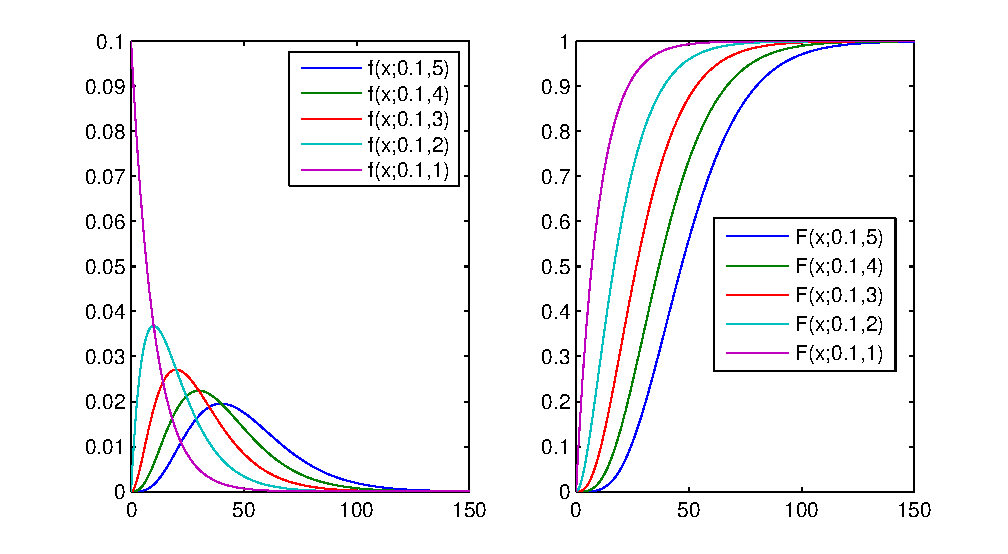
\includegraphics[width=6.50in]{figures/PlotPdfCdfGamma}}
\end{figure}


Note that if $X \sim \gammA(1,\beta)$ then $X \sim \exponential(\beta)$, since:
\[
f(x;1,\beta)  
= \frac{1}{(1-1)!}  \beta \exp(-\beta x) = \beta \exp(-\beta x) \ .
\]
More generally, if $X \sim \gammA(\alpha,\beta)$ and $\alpha \in \Nz$, then $X \sim \sum_{i=1}^{\alpha} Y_i$, where $Y_i \overset{IID}{\sim} \exponential(\beta)$ RVS, i.e.~ the sum of $\alpha$ IID $\exponential(\beta)$ RVs forms the model for the $\gammA(\alpha,\beta)$ RV.  If you model the inter-arrival time of buses at a bus-stop by IID $\exponential(\beta)$ RV, then you can think of the arrival time of the $k^{\text th}$ bus as a $\gammA(\alpha,\beta)$ RV.

%\section{Discrete Random Variables}
%}%end remove


%\remove{
\section*{Summary of Random Variables}\label{S:SummaryRVs}
\begin{table}[ht]
\centering
\begin{tabular}{|c|c|c|c|}%|c}
\hline
Model &PDF&Mean&Variance\\ \hline%&{\tt MGF}\\
%$\pointmass(\theta)$&$\BB{1}_{\{\theta\}}(x)$&$\theta$&$0$\\%&$e^{\theta t}$\\
$\bernoulli(\theta)$ &$\theta^x(1-\theta)^{1-x} \BB{1}_{\{0,1\}}(x)$&$\theta$&$\theta(1-\theta)$\\%&$\theta e^t+(1-\theta)$\\
$\binomial(n,\theta)$&$(^n_{\theta})\theta^x(1-\theta)^{n-x} \BB{1}_{\{0,1,\ldots,n\}}(x)$&$n \theta$&$n \theta(1-\theta)$\\%&$(\theta e^t+(1-\theta))^n$\\
$\geometric(\theta)$ &$\theta(1-\theta)^{x} \BB{1}_{\Zz_+}(x)$&$ \frac{1}{\theta}-1$&$\frac{1-\theta}{\theta^2}$\\%&$\frac{\theta e^t}{1-(1-\theta)e^t}(t<-log(1-\theta))$\\
$\poisson(\lambda)$&$\frac{\lambda^xe^{-\lambda}}{x!} \BB{1}_{\Zz_+}(x)$&$\lambda$&$\lambda$\\%&$e^{\lambda(e^t-1)}$\\
$\uniform(\theta_1,\theta_2)$&$\BB{1}_{[\theta_1,\theta_2]}(x)/(\theta_2-\theta_1)$&$\frac{\theta_1+\theta_2}{2}$&$\frac{(\theta_2-\theta_1)^2}{12}$\\%&$\frac{e^{\theta_2 t}-e^{\theta_1 t}}{(\theta_2-\theta_1)t}$\\
$\exponential(\lambda)$&$\lambda e^{-\lambda x}$&$\lambda^{-1}$&$\lambda^{-2}$\\%&$\frac{1}{1-\frac{1}{\lambda} t}(t<\lambda)$\\
$\normal(\mu,\sigma^2)$&$\frac{1}{\sigma\sqrt{2\pi}}e^{(x-\mu)^2/(2\sigma^2)}$&$\mu$&$\sigma^2$\\%&$exp\{ut+\frac{\sigma^2t^2}{2}\}$\\
$\gammA(\alpha,\beta)$&$\frac{\beta^{\alpha}}{\Gamma(\alpha)}{x^{\alpha-1}e^{-\beta x}}$&$\alpha/\beta$&$\alpha/\beta^2$\\%&$(\frac{1}{1-\beta t})^{\alpha}(t<1/\beta)$\\
%$\betA(\alpha,\beta)$ & $\frac{\Gamma(\alpha+\beta)}{\Gamma(\alpha)\Gamma(\beta)}x^{\alpha-1}(1-x)^{\beta-1}$ & $\frac{\alpha}{\alpha+\beta}$ & $\frac{\alpha\beta}{(\alpha+\beta)^2 (\alpha+\beta+1)} $ \\%& $ 1+\Sigma^\infty_{k+1}(\Pi^{k-1}_{r=0}\frac{\alpha+r}{\alpha+\beta+r})\frac{t^k}{k\!}$\\
%$t_v$ & $\frac{\Gamma((v+1)/2)}{\Gamma(v/2)}  \frac{1}{(1+x^2/v)^{(v+1)/2}$ &0 (if $v>1$ ) & $\frac{v}{v-2}$  (if $v>2$) & does not exist \\
% $\chi^2_p$&$\frac{1}{\Gamma(p/2)2^{p/2}}x^{(p-2)-1}e^{-x/2}$&$p$&$2p$\\ \hline%&$(\frac{1}{1-2t})^{p/2}(t<1/2)$\\
\hline
\end{tabular}
\caption{Random Variables with PDF, Mean and Variance}
%\label{tab:}
\end{table}


We need a new notion for the variance of two RVs.
\begin{definition}[Covariance]
Suppose $X_1$ and $X_2$ are random variables, such that $\e(X_1^2) < \infty$ and $\e(X_2)^2 < \infty$.  Then, $\e(|X_1 X_2|) < \infty$ and $\e(|(X_1-\e(X_1))(X_2-\e(X_2))|) < \infty$.  We therefore define the covariance $\cv(X_1,X_2)$ of $X_1$ and $X_2$ as:
\[
\cv(X_1,X_2) := \e \left((X_1-\e(X_1))(X_2-\e(X_2))\right) = \e(X_1 X_2) - \e(X_1) \e(X_2)
\]
\end{definition}

Let us consider the natural two-dimensional analogue of the $\bernoulli(\theta)$ RV in the real plane $\Rz^2 := (-\infty,\infty)^2 := (-\infty,\infty) \times (-\infty,\infty)$.  A natural possibility is to use the {\bf ortho-normal basis vectors} in $\Rz^2$:
$$ \boxed{
e_1 := (1,0), \qquad e_2 := (0,1)
} \ .$$
Recall that vector addition and subtraction are done component-wise, i.e.~$(x_1,x_2) \pm (y_1,y_2) = (x_1\pm y_1,x_2 \pm y_2)$.

\begin{classwork}[Geometry of Vector Addition]
Recall elementary vector addition in the plane.  What is $(1,0)+(1,0)$, $(1,0)+(0,1)$, $(0,1)+(0,1)$?  What is the relationship between $(1,0)$, $(0,1)$ and $(1,1)$ geometrically? How does the diagonal of the parallelogram relate the its two sides in the geometry of addition in the plane?  What is  $(1,0)+(0,1)+(1,0)$?
\end{classwork}

\begin{figure}[htpb]
\caption{Quincunx on the Cartesian plane.  Simulations of $\binomial(n=10,\theta=0.5)$ RV as the x-coordinate of the ordered pair resulting from the culmination of sample trajectories formed by the accumulating sum of $n=10$ IID $\bernoulli(\theta=0.5)$ random vectors over $\{(1,0),(0,1)\}$ with probabilities $\{\theta,1-\theta\}$, respectively.  The blue lines and black asterisks perpendicular to and above the diagonal line, i.e.~the line connecting $(0,10)$ and $(10,0)$, are the density histogram of the samples and the PDF of our $\binomial(n=10,\theta=0.5)$ RV, respectively.\label{F:BinomQuincunxn10r10r1000}}
\centering
\mbox{\subfigure[Ten samples]{\hspace{-2cm} \includegraphics[width=3.250in]{figures/BinomQuincunxn10r10}} \hspace{-2cm}
	   \subfigure[Thousand samples]{\includegraphics[width=3.250in]{figures/BinomQuincunxn10r1000}} }
\end{figure}

\begin{model}[$\bernoulli(\theta)$ \rv]
Given a parameter $\theta \in [0,1]$, we say that $X := (X_1,X_2)$ is a $\bernoulli(\theta)$ random vector (\rv) if it has only two possible outcomes in the set $\{e_1,e_2\} \subset \Rz^2$, i.e.~$x:=(x_1,x_2) \in \{(1,0),(0,1)\}$.  The PMF of the \rv~$X:= (X_1,X_2)$ with realisation $x:=(x_1,x_2)$ is:
\[
f(x;\theta) := \p(X=x) = \theta \, \BB{1}_{\{e_1\}}(x) + (1-\theta) \, \BB{1}_{\{e_2\}}(x) =
\begin{cases}
\theta & \text{if } \quad x=e_1:=(1,0) \\
1- \theta & \text{if } \quad x=e_2:=(0,1) \\
0 & \text{otherwise}
\end{cases}
\]
\end{model}


\begin{classwork}[Expectation and Variance of $\bernoulli(\theta)$ \rv]
What is the Expectation of $\bernoulli(\theta)$ \rv?
\[
\e_{\theta}(X) = \e_{\theta}((X_1,X_2)) = \sum_{(x_1,x_2) \in \{e_1,e_2\}} (x_1,x_2) f((x_1,x_2);\theta) = (1,0) \theta + (0,1) (1-\theta) = (\theta,1-\theta) \ .
\]

How about the variance ? [Hint: Use the definitions of $\e(X)$ and $\V(X)$ for the \rv~$X$.  $\e(X^2)$ is not a single number and you may need new words such as covariance to deal with terms like $\e(X_1 X_2)$.]
\end{classwork}

%\remove{
We can write the $\binomial(n,\theta)$ RV $Y$ as a $\binomial(n,\theta)$ \rv~$X:=(Y,n-Y)$.  In fact, this is the underlying model and the {\bf bi} in the $\binomial(n,\theta)$ does refer to two in Latin.  In the coin-tossing context this can be thought of keeping track of the number of Heads and Tails out of an IID sequence of $n$ tosses of a coin with probability $\theta$ of observing Heads.  In the Quincunx context, this amounts to keeping track of the number of right and left turns made by the ball as it drops through $n$ levels of pegs where the probability of a right turn at each peg is independently and identically $\theta$.  In other words, the $\binomial(n,\theta)$ \rv~$(Y,n-Y)$ is the sum of $n$ IID $\bernoulli(\theta)$ {\rv}s $X_1:=(X_{1,1},X_{1,2}), X_2:=(X_{2,1},X_{2,2}), \ldots, X_n:=(X_{n,1},X_{n,2})$:
\[
(Y,n-Y) = X_1+X_2+\cdots + X_n = (X_{1,1},X_{1,2}) + (X_{2,1},X_{2,2}) + \cdots + (X_{n,1},X_{n,2})
\]

Go the Biomathematics Research Centre on the 6th floor of Erskine to play with the Quincunx built by Ryan Lawrence in 2007 (See the project by Ashman and Lawrence at  \href{http://www.math.canterbury.ac.nz/~r.sainudiin/courses/STAT218/projects/Stat218StudentProjects2007.pdf}{\url{http://www.math.canterbury.ac.nz/~r.sainudiin/courses/STAT218/projects/Stat218StudentProjects2007.pdf}} % \ref{S:AshmanLawrenceQuincunx} 
for details).  It is important to gain a physical intimacy with the Quincunx to appreciate the following model of it.  We can make a statistical model of Galton's observations earlier regarding the dynamics of lead shots through the Quincunx as the sum of $n$ IID $\bernoulli(0.5)$ \rv{s}, where $n$ is number of pegs that each ball bounces on before making a left or right turn with equal probability.  

\begin{exercise}[Number of paths and the binomial coefficient]
How does the number of paths that lead to a bucket $(x_1,x_2)$ with $x_1+x_2=n$ relate to the binomial coefficient $\binom{n}{x_1} ?$
%\vspace{2cm}
\end{exercise}

\begin{labwork}[Quincunx Sampler Demo -- Sum of $n$ IID $\bernoulli(1/2)$ \rv{s}]\label{LW:QuincunxSampler}
Let us understand the Quincunx construction of the $\binomial(n,1/2)$ \rv $X$ as the sum of $n$ independent and identical $\bernoulli(1/2)$ \rv{s} by calling the interactive visual cognitive tool as follows:
\begin{VrbM}
>> guiMultinomial
\end{VrbM}
The M-file {\tt guiMultinomial.m} will bring a graphical user interface (GUI) as shown in \hyperref[F:guiMultinomialQuincunx]{Figure \ref*{F:guiMultinomialQuincunx}}.  Using the drop-down menu at ``How many levels?'' change the number of levels to $2$ ($n=2$).  Now click the ``Do one'' button as many times as you like and comprehend the simulation process -- the path taken by the ball as it falls through two levels.  Next, from the drop-down menu at ``How many  Replication?'' change it from $10$ to $100$.  You can press ``Do all'' to watch all 100 balls drop into their possible values at level $2$.  Change the number of levels or $n$ in $\binomial(n,1/2)$ \rv to $3$ or $5$ or $10$ and do more simulations until you are comfortable with the construction that the sum of $n$ IID $\bernoulli(1/2)$ \rv{s} is the $\binomial(n,1/2)$ \rv.

When we drop $1000$ balls into the simulated Quincunx the density histogram is much closer to the PDF of $\binomial(n=10,\theta=0.5)$ RV than when we only drop $10$ balls.  See \hyperref[F:BinomQuincunxn10r10r1000]{Figure \ref*{F:BinomQuincunxn10r10r1000}} for a description of the simulations.  Try to replicate such a simulation on your own.
\end{labwork}

\begin{figure}[htpb]
\caption{Visual Cognitive Tool GUI: Quincunx.\label{F:guiMultinomialQuincunx}}
\centering   \makebox{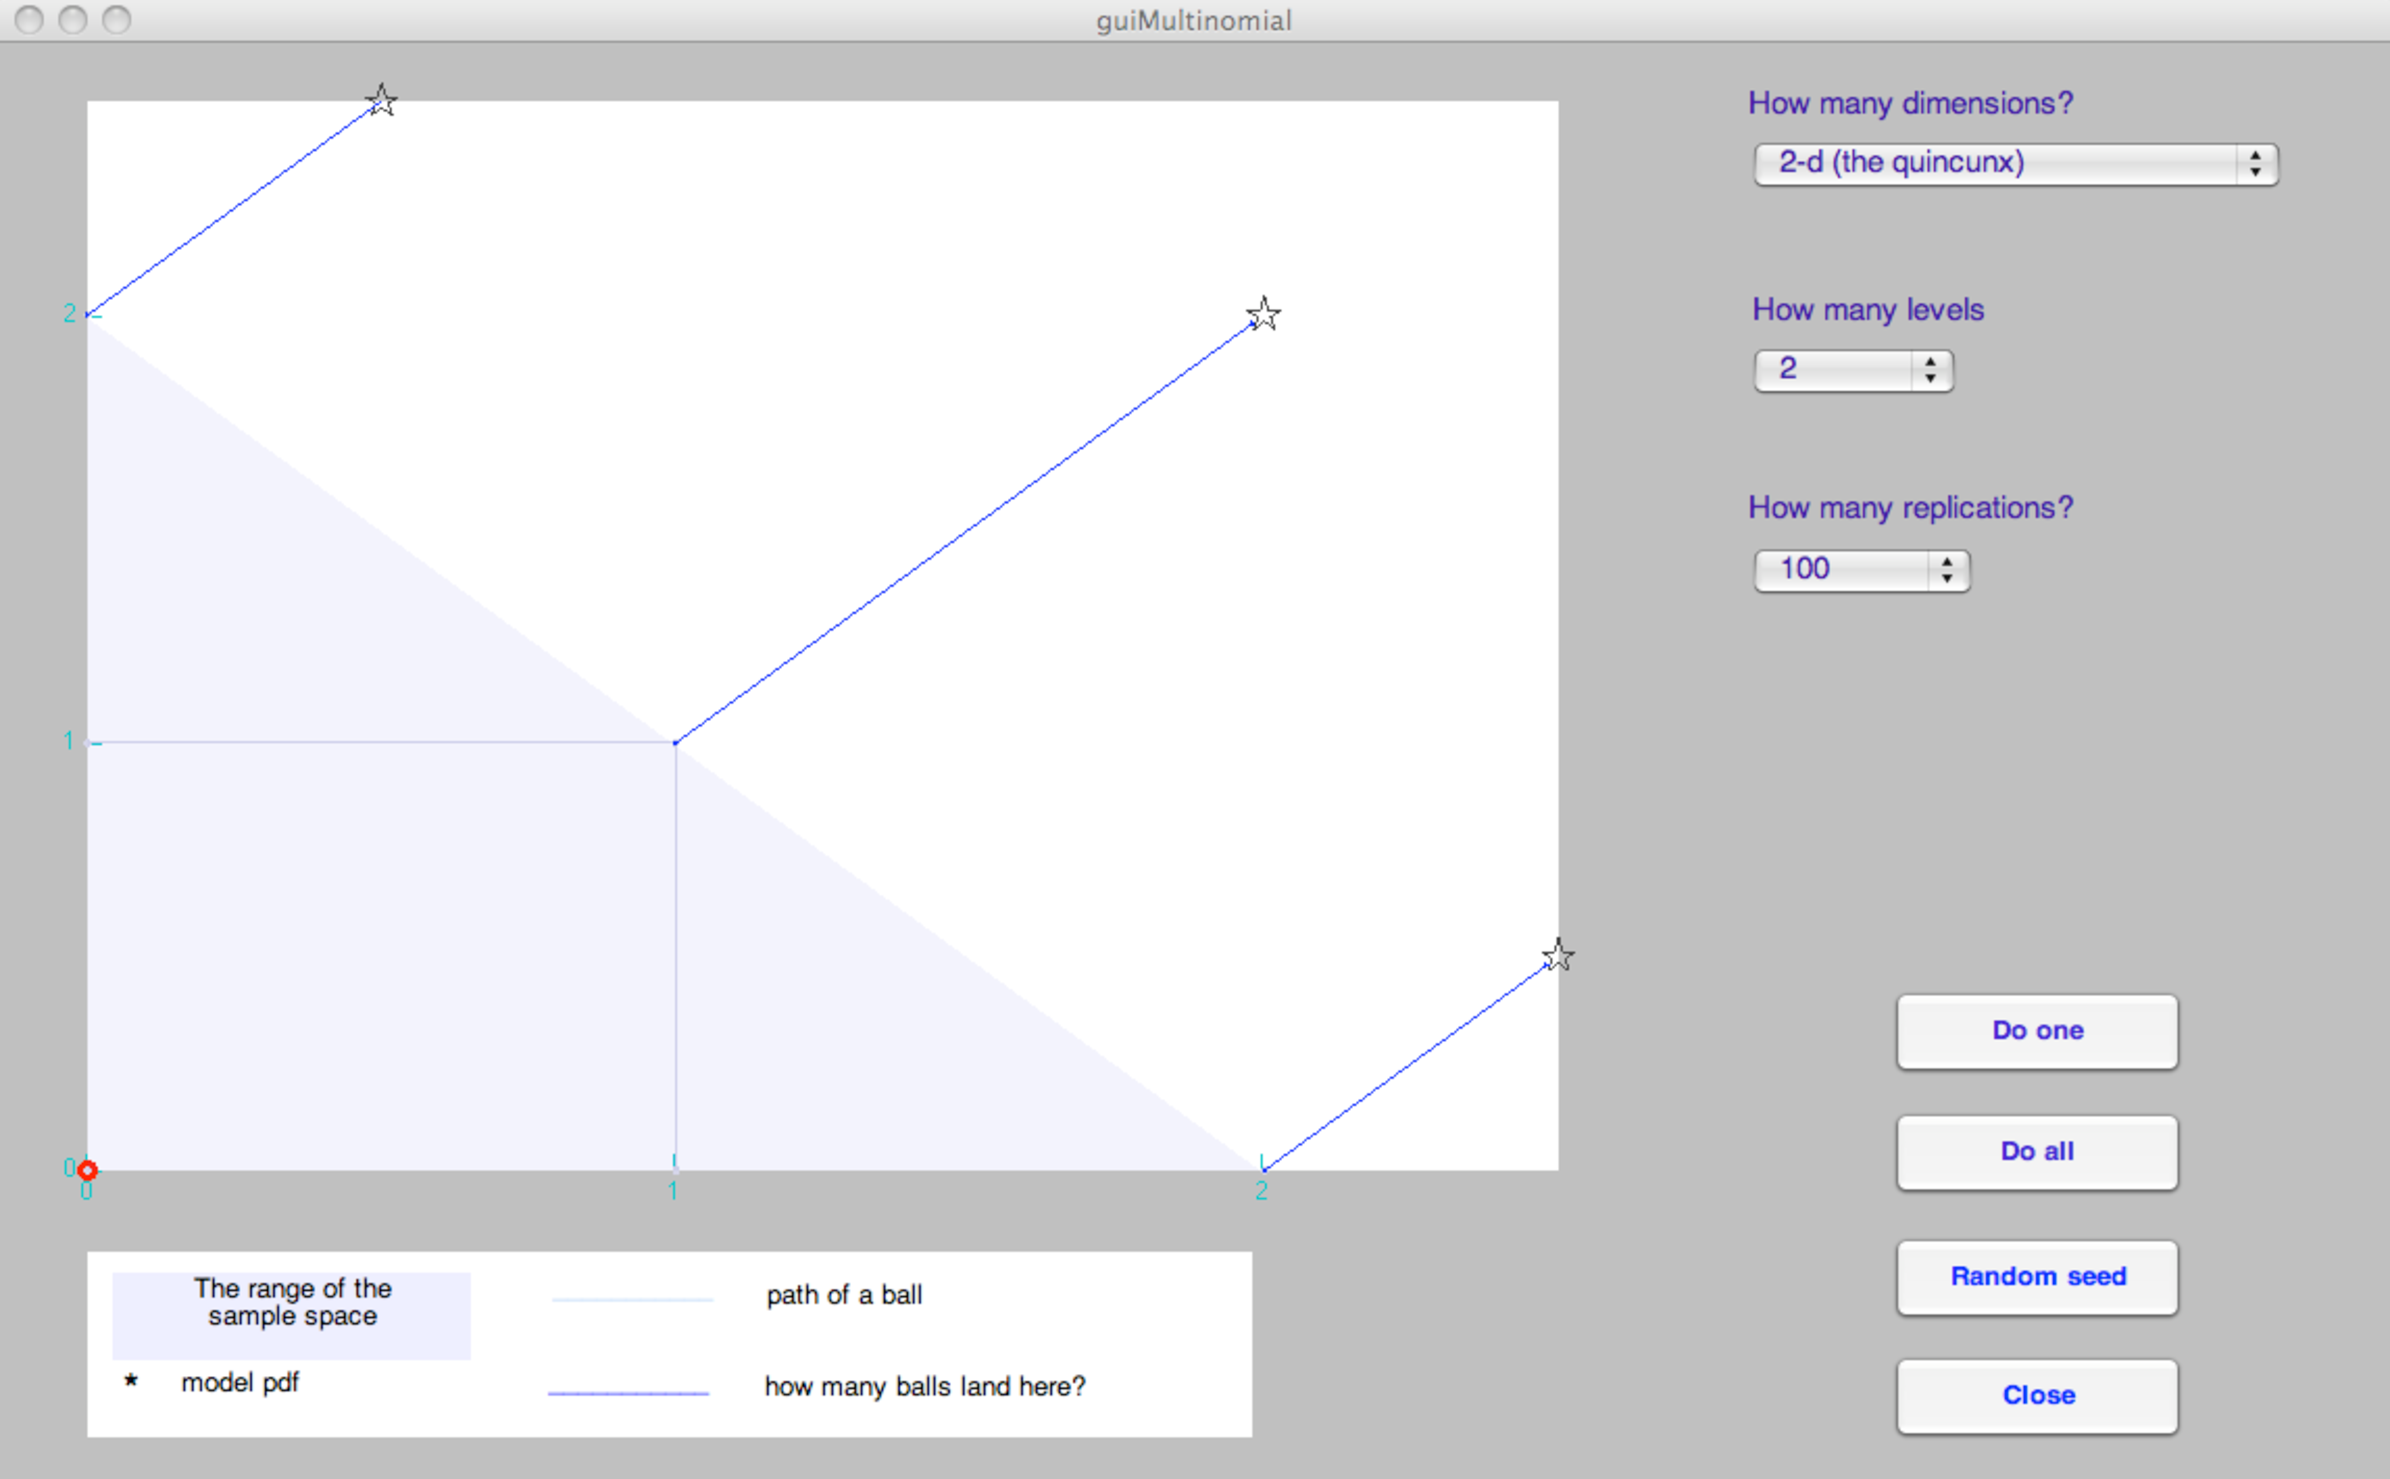
\includegraphics[width=6.50in]{figures/guiMultinomialQuincunx}}
\end{figure}
%}%end remove

We are now ready to extend the $\binomial(n,\theta)$ RV or \rv~to its multivariate version called the $\multinomial(n,\theta_1,\theta_2,\ldots,\theta_k)$ \rv.  We develop this \rv~as the sum of $n$ IID $\demoivre(\theta_1,\theta_2,\ldots,\theta_k)$ \rv~that is defined next.

\begin{model}[$\demoivre(\theta_1,\theta_2,\ldots,\theta_k)$ \rv]\label{M:deMoivreRVec}
The PMF of the $\demoivre(\theta_1,\theta_2,\ldots,\theta_k)$ \rv~$X := (X_1,X_2,\ldots,X_k)$ taking value $x := (x_1,x_2,\ldots,x_k) \in \{e_1,e_2,\ldots,e_k\}$, where the $e_i$'s are ortho-normal basis vectors in $\Rz^k$ is:
\[
f(x;\theta_1,\theta_2,\ldots,\theta_k) := \p(X=x) = \sum_{i=1}^k \theta_i \BB{1}_{\{e_i\}}(x) =
\begin{cases}
\theta_1 & \text{if} \quad x=e_1:=(1,0,\ldots,0) \in \Rz^k \\
\theta_1 & \text{if} \quad x=e_1:=(0,1,\ldots,0) \in  \Rz^k \\
\vdots \\
\theta_k & \text{if} \quad x=e_k:=(0,0,\ldots,1) \in  \Rz^k \\
0 & \text{otherwise}
\end{cases}
\]
Of course, $\sum_{i=1}^k \theta_i = 1$.
\end{model}

When we add $n$ IID $\demoivre(\theta_1,\theta_2,\ldots,\theta_k)$ \rv~together, we get the $\multinomial(n,\theta_1,\theta_2,\ldots,\theta_k)$ \rv~as defined below.

\begin{model}[$\multinomial(n,\theta_1,\theta_2,\ldots,\theta_k)$ \rv]\label{M:Multinomial}
We say that a \rv~$Y:=(Y_1,Y_2,\ldots,Y_k)$ obtained from the sum of $n$ IID $\demoivre(\theta_1,\theta_2,\ldots,\theta_k)$ \rv{s} with realisations
$$y:=(y_1,y_2,\ldots,y_k) \in \Yz:= \{(y_1,y_2,\ldots,y_k) \in \Zz_+^k : \sum_{i=1}^k y_i = n\}$$ has the PMF given by:
\[
f(y;n,\theta) := f(y;n,\theta_1,\theta_2,\ldots,\theta_k) := \p(Y=y;n,\theta_1,\theta_2,\ldots,\theta_k) = \binom{n}{y_1,y_2,\ldots,y_k} \prod_{i=1}^k \theta_i^{y_i} \ ,
\]
where, the multinomial coefficient:
\[
 \binom{n}{y_1,y_2,\ldots,y_k} := \frac{n!}{y_1! y_2! \cdots y_k!} \ .
\]
Note that the marginal PMF of $Y_j$ is $\binomial(n,\theta_j)$ for any $j=1,2,\ldots,k$.
\end{model}

\begin{figure}[htpb]
\caption{Septcunx on the Cartesian co-ordinates.  Simulations of $\multinomial(n=2,\theta_1=1/3,\theta_2=1/3,\theta_3=1/3)$ \rv~as the sum of $n$ IID $\demoivre(\theta_1=1/3,\theta_2=1/3,\theta_3=1/3)$ \rv{s} over $\{(1,0,0),(0,1,0),(0,0,1)\}$ with probabilities $\{\theta_1,\theta_2,\theta_3\}$, respectively.  The blue lines perpendicular to the sample space of the $\multinomial(3,\theta_1,\theta_2,\theta_3)$ \rv, i.e.~the plane in $\Rz^3$ connecting $(n,0,0)$, $(0,n,0)$ and $(0,0,n)$, are the density histogram of the samples.\label{F:MultinomSeptcunxn2n10r1000}}
\centering
\mbox{\subfigure[Thousand Samples with $n=2$]{\hspace{-2cm} 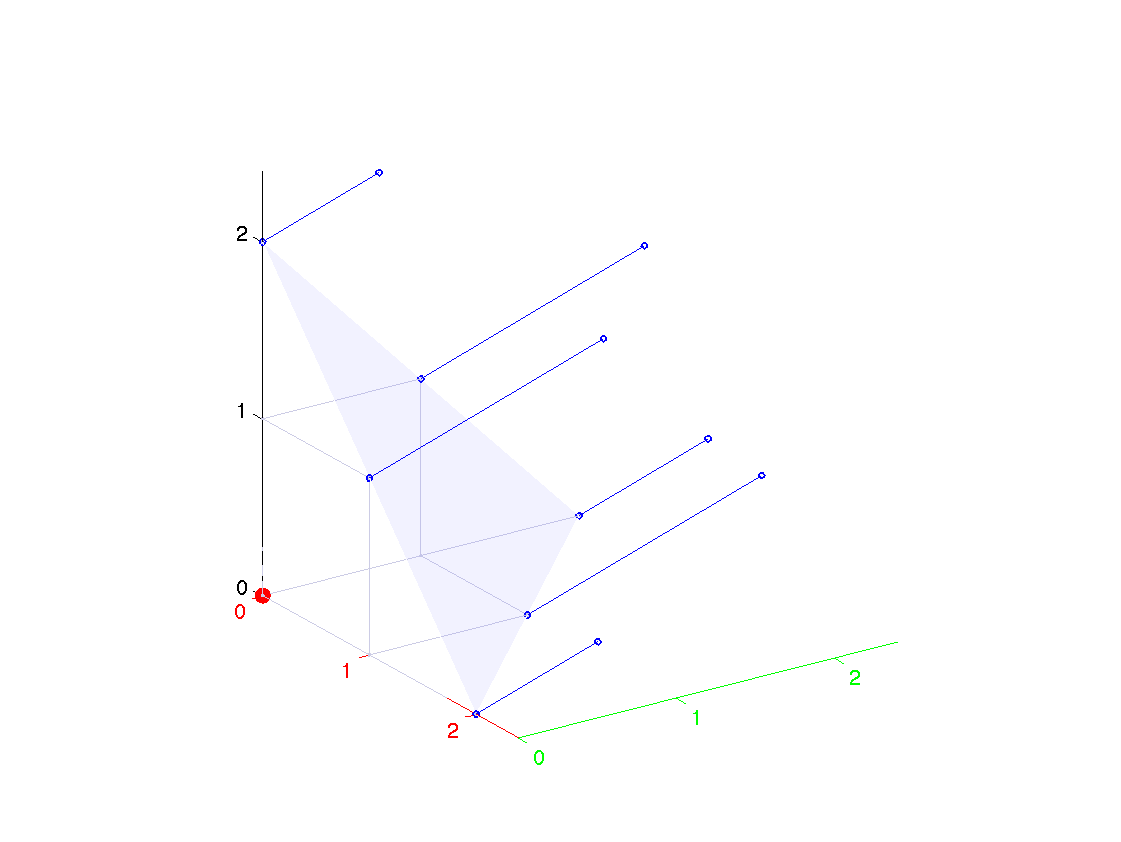
\includegraphics[width=4.250in]{figures/MultinomSeptcunxn2r1000}} \hspace{-2cm}
	   \subfigure[Thousand Samples with $n=10$]{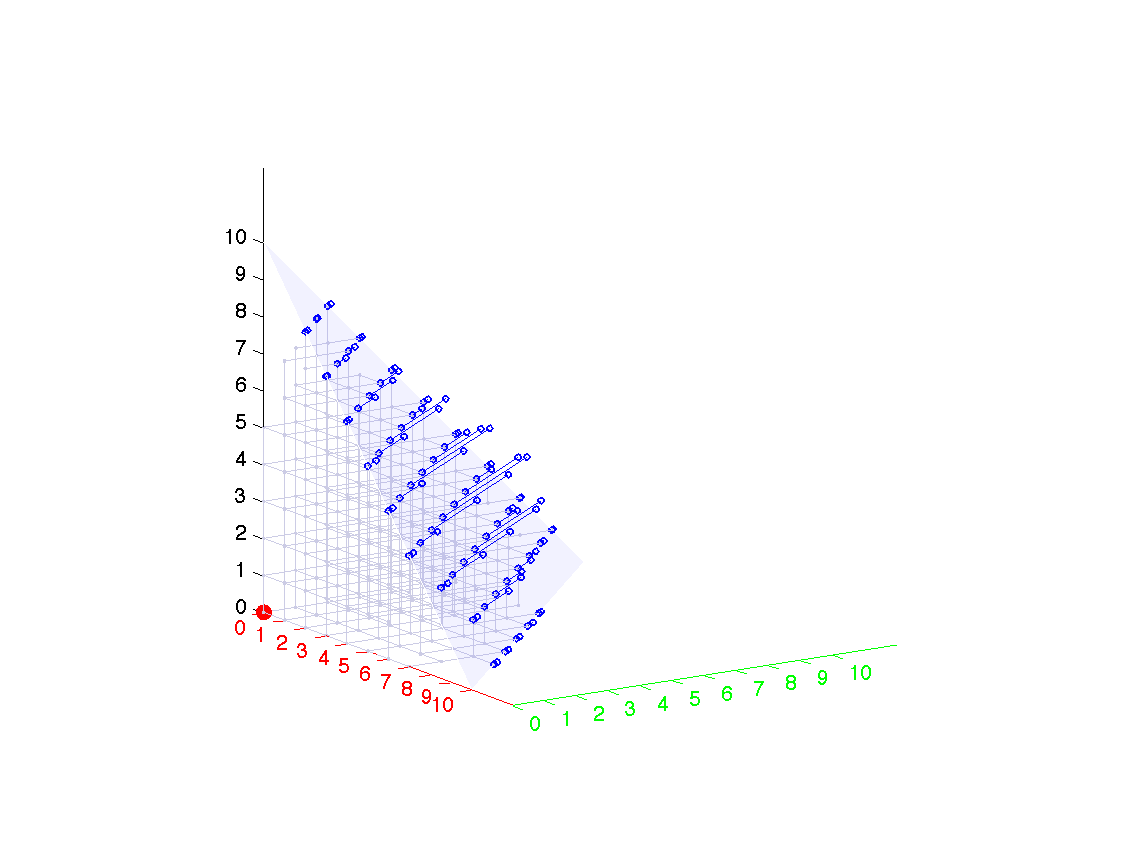
\includegraphics[width=4.250in]{figures/MultinomSeptcunxn10r1000}} }
\end{figure}

We can visualise the $\multinomial(n,\theta_1,\theta_2,\theta_3)$ process as a sum of $n$ IID $\demoivre(\theta_1,\theta_2,\theta_3)$ \rv{s} via a three dimensional extension of the Quincunx called the ``Septcunx'' and relate the number of paths that lead to a given trivariate sum $(y_1,y_2,y_3)$ with $\sum_{i-1}^3 y_i = n$ as the multinomial coefficient $\frac{n!}{y_1! y_2! y_3!}$.  In the Septcunx, balls choose from one of three paths along $e_1$, $e_2$ and $e_3$ with probabilities $\theta_1$, $\theta_2$ and $\theta_3$, respectively, in an IID manner at each of the $n$ levels, before they collect at buckets placed at the integral points in the $3$-simplex, $\Yz = \{(y_1,y_2,y_3) \in \Zz_+^3 : \sum_{i=1}^3 y_i=n \}$.  Once again, we can visualise that the sum of $n$ IID $\demoivre(\theta_1,\theta_2,\theta_3)$ \rv{s} constitute the $\multinomial(n,\theta_1,\theta_2,\theta_3)$ \rv~as depicted in \hyperref[F:MultinomSeptcunxn2n10r1000]{Figure \ref*{F:MultinomSeptcunxn2n10r1000}}.

%\remove{
\begin{labwork}[Septcunx Sampler Demo -- Sum of n IID $\demoivre(1/3,1/3,13/)$ \rv{s}]\label{LW:SeptcunxSampler}
Let us understand the Septcunx construction of the $\multinomial(n,1/3,1/3,1/3)$ \rv $X$ as the sum of $n$ independent and identical $\demoivre(1/3,1/3,13/)$ \rv{s} by calling the interactive visual cognitive tool as follows:
\begin{VrbM}
>> guiMultinomial
\end{VrbM}
The M-file {\tt guiMultinomial.m} will bring a GUI as shown in \hyperref[F:guiMultinomialQuincunx]{Figure \ref*{F:guiMultinomialQuincunx}}.  Using the drop-down menu at ``How many dimensions?'' change to ``3-d (the septcunx)'' and you will see a septcunx as shown in \hyperref[F:guiMultinomialSeptcunx]{Figure \ref*{F:guiMultinomialSeptcunx}}.  Next, using the drop-down menu at ``How many levels?'' change the number of levels to $2$ ($n=2$).  Now click the ``Do one'' button as many times as you like and comprehend the simulation process -- the path taken by the ball as it falls through two levels in three dimensional space.  Feel free to change the up-down and left-right sliders for the view angles.  Next, from the drop-down menu at ``How many  Replication?'' change it from $10$ to $100$.  You can press ``Do all'' to watch all 100 balls drop into their possible values at level $2$.  Change the number of levels or $n$ in $\multinomial(n,1/3,1/3,1/3)$ \rv to $5$ or $10$ and do more simulations until you are comfortable with the construction that the sum of $n$ IID $\demoivre(1/3,1/3,1/3)$ \rv{s} is the $\multinomial(n,1/3,1/3,1/3)$ \rv.
\end{labwork}

\begin{figure}[htpb]
\caption{Visual Cognitive Tool GUI: Septcunx.\label{F:guiMultinomialSeptcunx}}
\centering   \makebox{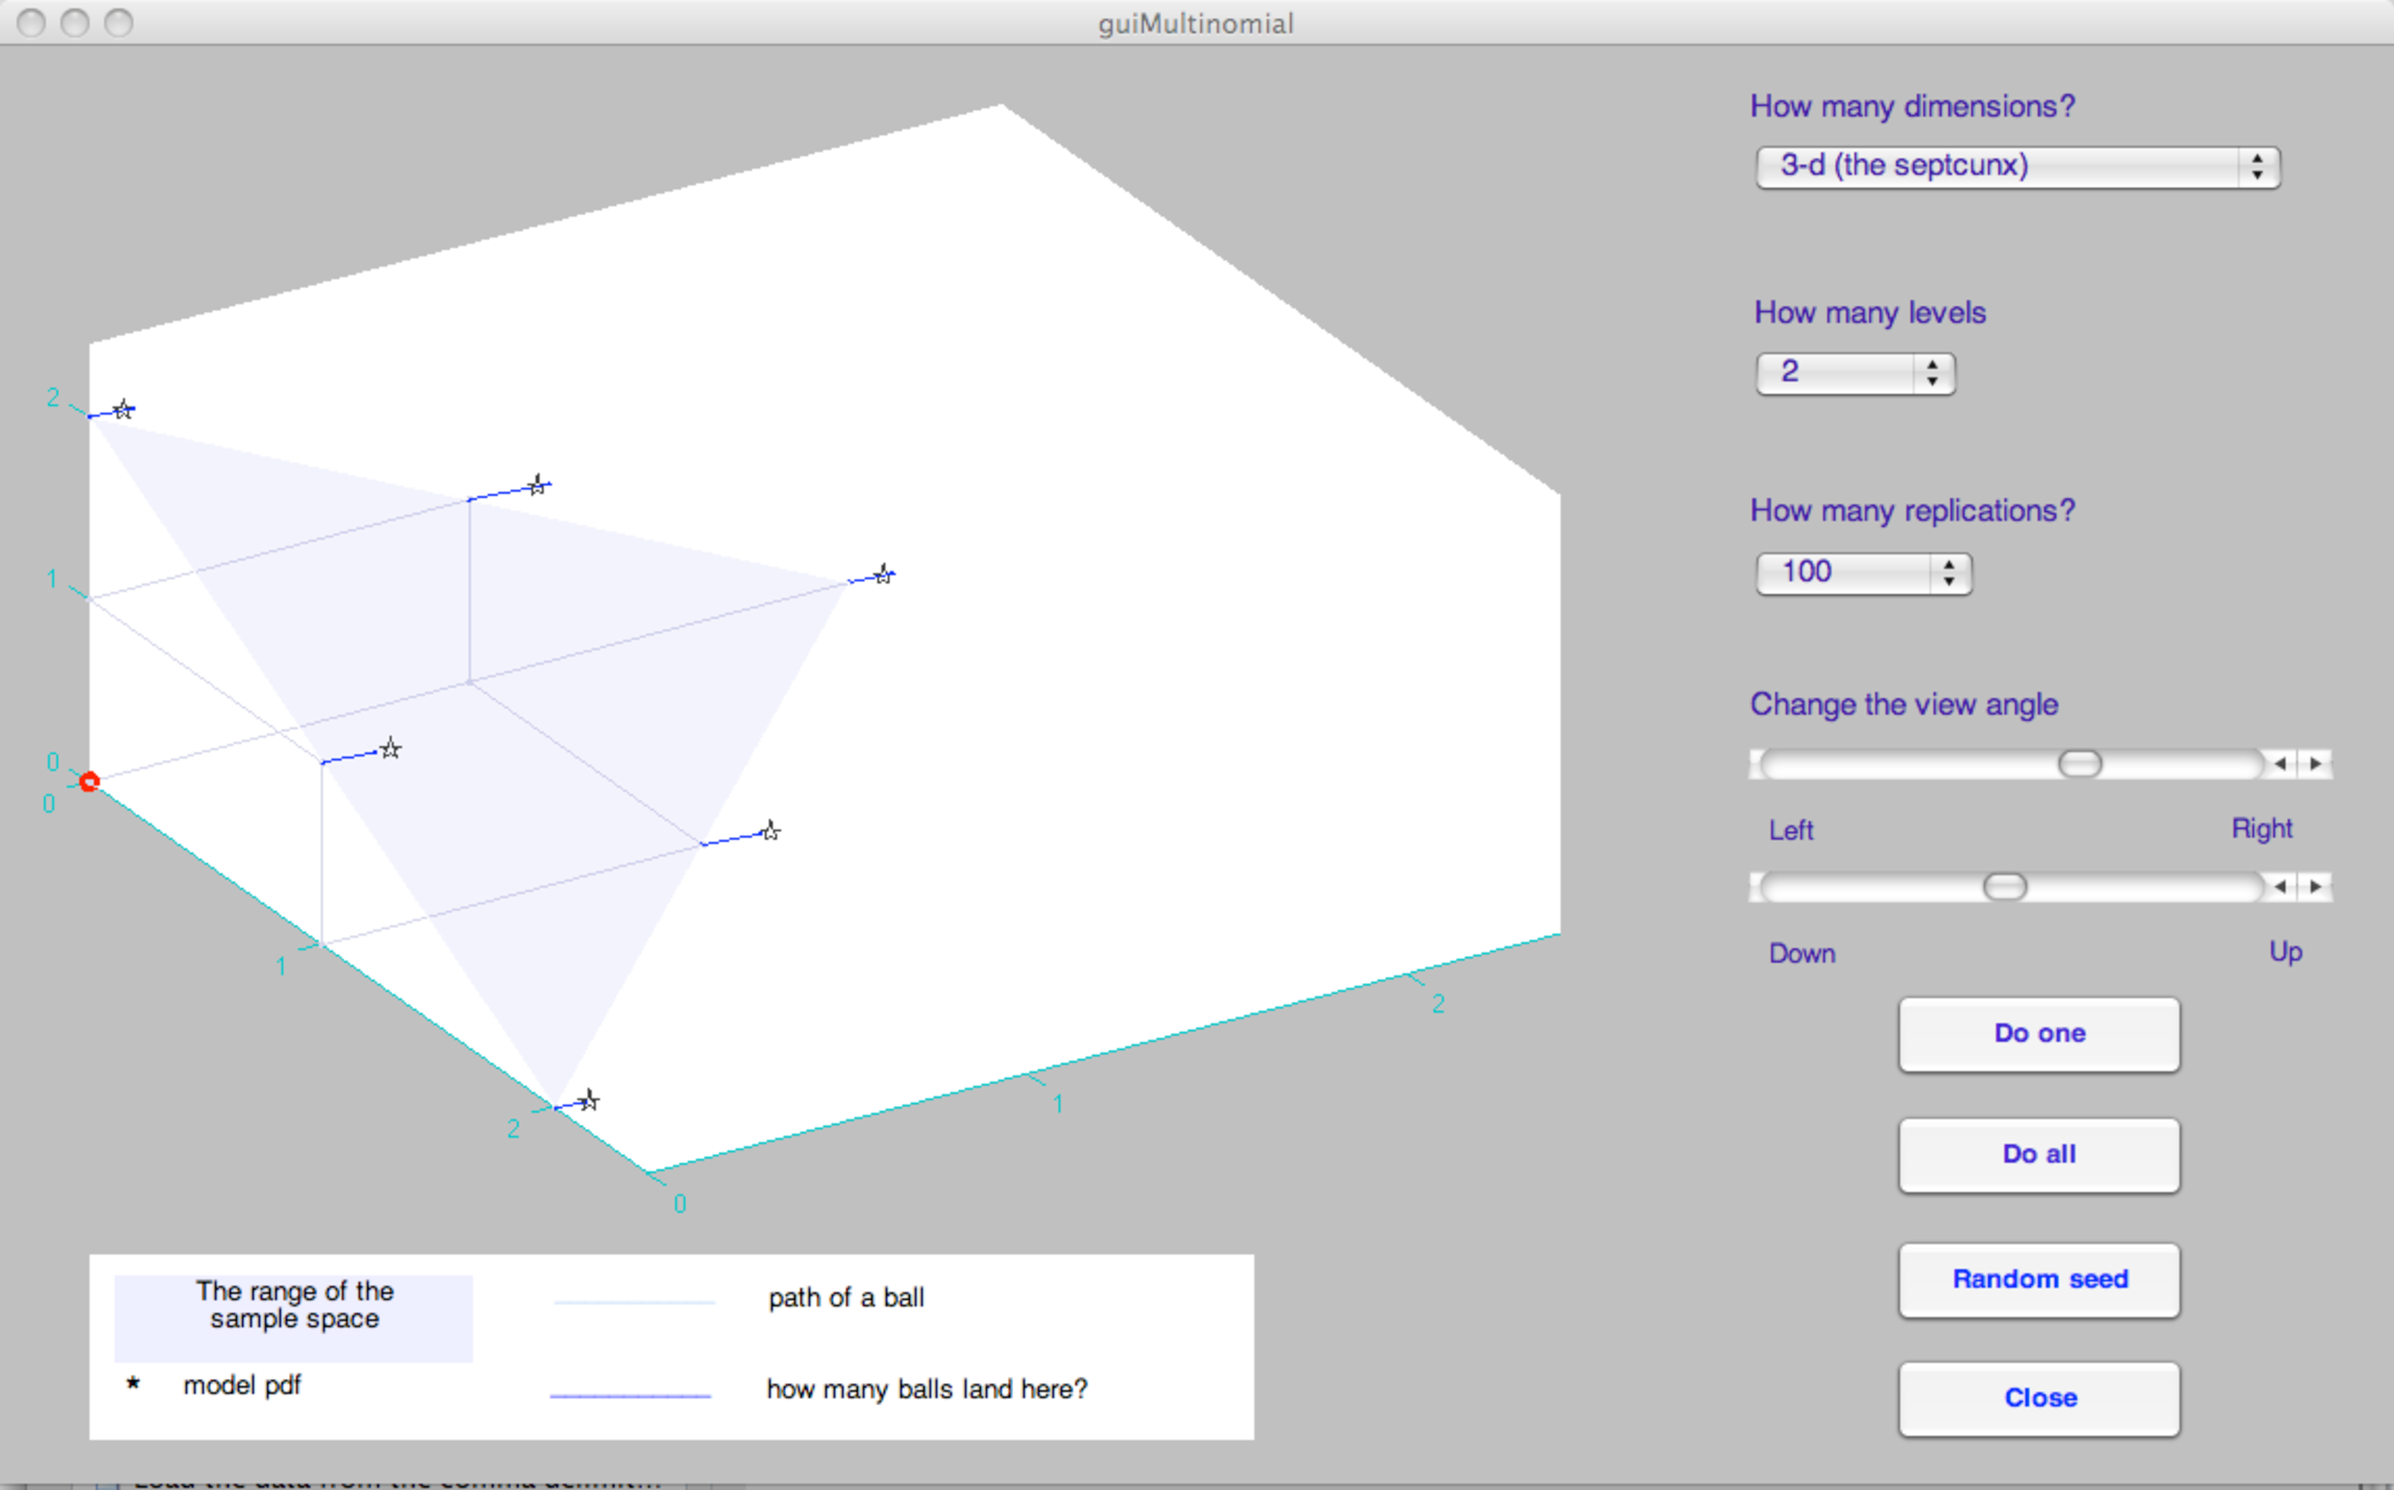
\includegraphics[width=6.50in]{figures/guiMultinomialSeptcunx}}
\end{figure}


\begin{labwork}[PDF of $\multinomial(n,\theta)$ \rv]\label{LW:MultinomialPdf}
We can implement the following \Matlab function {\tt MultinomialPdf} to compute the PDF of the $\multinomial(n,\theta)$ \rv~where $\theta:=(\theta_1,\theta_2,\ldots,\theta_k)$ is a point in the $k$-simplex $\bigtriangleup_k$ as follows:
\VrbMf[label=MultinomialPdf.m]{scripts/MultinomialPdf.m}
We can call this function to evaluate the PDF at a specific sample $x=(x_1,x_2,\ldots,x_k)$ as follows:
\begin{VrbM}
>> MultinomialPdf([2 0 0],2,[1/3 1/3 1/3])
ans =    0.1111
>> MultinomialPdf([0 2 0],2,[1/3 1/3 1/3])
ans =    0.1111
>> MultinomialPdf([0 0 2],2,[1/3 1/3 1/3])
ans =    0.1111
>> MultinomialPdf([1 1 0],2,[1/3 1/3 1/3])
ans =    0.2222
>> MultinomialPdf([1 0 1],2,[1/3 1/3 1/3])
ans =    0.2222
>> MultinomialPdf([0 1 1],2,[1/3 1/3 1/3])
ans =    0.2222
\end{VrbM}
\end{labwork}

\begin{simulation}[A simple multinomial simulation]\label{SIM:Multinomial}
Using the identity matrix $I$ in $\Rz^3$ that can be created in \Matlab using the {\tt eye(3)} command, and the $\demoivre(1/3,1/3,1/3)$ RV sampler, simulate vector-valued samples from $\demoivre(1/3,1/3,1/3)$ \rv.  Finally add up $n=10$ samples from $\demoivre(1/3,1/3,1/3)$ \rv~to produce samples from $\multinomial(10,1/3,1/3,1/3)$ \rv.
\end{simulation}

%%% begin Dominic's Material
%%% WORK: We need to introduce sampling from a large discrete distribution, say the Alias method before this material % theoretically explain randsample function in Matlab
\remove{
\section{Importance Resampler}
The rejection method cannot be used when the constant $a$ or $\tilde{a}$ that guarantees the envelape condition cannot be found. The importance resampler, also known as the method of {sampling/importance resampling}, does not require the constant, but it produces a random variable that is only approximately distributed according to $f$. As for the rejection method, we need a density/mass function $g$ that we can generate from and that has support at least as large as the support of $f$.

\begin{algorithm}
\caption{Importance Resampler}
\label{A:ImpReSampler}
\begin{algorithmic}[1]
\STATE {
{\it input:}
\begin{itemize}
\item[(1)] shape of a target density $\tilde{f}(x) = \left({\int \tilde{f}(x)dx}\right) f(x)$,
\item[(2)] a proposal density $g(x)$ satisfying only (a) and (b) above.
\item[(3)] a large enough integer $m$.
\end{itemize}
}
\STATE {\it output:} a sample $x{\prime}$ from RV $X^{\prime}$ with density $f^{\prime}$ that is close to  $f$
\STATE Generate $y_1,\ldots, y_m \sim g$
\STATE Compute
$$
w_i=\frac{f(y_i)/g(y_i)}{\sum^m_{j=1}f(y_j)/g(y_j)},i=1,\ldots,m \enspace .
$$
\STATE Resample $x^{\prime}$ from $\{y_1,\ldots, y_m\}$ with weights $\{w_1,\ldots, w_m\}$
\end{algorithmic}
\end{algorithm}

\begin{prop}The Importance Resampler of Algorithm~\ref{A:ImpReSampler} produces samples from a variable $X^{\prime}$ that is approximately distributed according to $f$, in the sense that:
\begin{equation}
\lim_{m\rightarrow \infty}\p( X^{\prime} \leq t)=\int^t_{-\infty}f(x)dx
\end{equation}
for any real number $t$.
\begin{proof}
\begin{displaymath}
\begin{split}
&\p(X^{\prime}\leq t)=\sum^m_{i=1}w_iI_{(-\infty,t]}(y_i)=\frac{\frac{1}{m}\sum^m_{i=1}\frac{f(y_i)}{g(y_i)}I_{(-\infty,t]}(y_i)}{\frac{1}{m}\sum^m_{i=1}\frac{f(y_i)}{g(y_i)}}\\
%\end{displaymath}
%\begin{displaymath}
&\underrightarrow{^{m\rightarrow\infty}}\frac{E [\frac{f(y)}{g(y)}I_{(-\infty,t]}(y)]}{E[\frac{f(y)}{g(y)}]}=\frac{\int^t_{-\infty}f(y)dy}{{\int^{\infty}_{-\infty}f(y)dy}}=\int^t_{-\infty}f(y)dy\\
\end{split}
\end{displaymath}
\end{proof}
\end{prop}

Let us visualise the Importance Resampler in action from \hyperref[Mf:ImpResamplerCauchyViaNormal]{Labwork~\ref*{Mf:ImpResamplerCauchyViaNormal}}.

\begin{labwork}[$\cauchy$ RV via Importance Resampler]
Use the sampling/importance resampling method to generate $1000$ approximate $\cauchy$ samples  by using the $\normal(0,1)$ samples:

$$f(x)=\frac{1}{\pi(1+x^2)} \textrm{ and  } g(x)=\frac{1}{\sqrt{2\pi}}\exp\left(-\frac{x^2}{2}\right).$$

\begin{VrbM}
n = 1000;
m = 10000;
y = randn(1,m); % randn is the N(0,1) generator in Matlab
y2 = y .* y;
w = exp(0.5 * y2) ./ (1 + y2);
w = w / sum(w);
x = randsample(y,n,true,w); % resample n values from y weighted by w
\end{VrbM}
\end{labwork}

Note that to get $n$ sample points from $f$ using sampling/importance resampling, we must start with a sample from $g$ of size $m$ larger than $n$.

As for the rejection method, the sampling/importance resampling method can still be used if only the un-normalised form of $f$ or $g$ (or both) is known, simply by using the un-normalised densities/mass functions to compute the weights.
%%%%%%end Dominic's material
}

\section{Other Continuous Random Variables}\label{S:OtherContRVs}
Here, we see other common continuous RVs that can be simulated from transforming RVs we have already encountered.
%}%end remove
%\remove{
\begin{simulation}[$\gammA(\lambda,k)$ for integer $k$]\label{SIM:Gamma}
Using this relationship we can simulate from $X \sim \gammA(\lambda,k)$, for an integer-valued $k$, by simply summing $k$ IID samples from $\exponential(\lambda)$ RV as follows:
\begin{VrbM}
>> lambda=0.1; %declare some lambda parameter
>> k=5; % declare some k parameter (has to be integer)
>> rand('twister',7267); % initialise the fundamental sampler
>> % sum k IID Exponential(lambda) samples for one desired sample from Gamma(lambda,k)
>> x= sum(-1/lambda*log(rand(k,1)))
x =   28.1401
>> % sum the 10 columns of k X 10 IID Exponential(lambda) samples for 10 desired samples from Gamma(lambda,k)
>> x= sum(-1/lambda*log(rand(k,10)))
x =
   83.8150   61.2674   80.3683  103.5748   48.4454   20.2269   93.8310   56.1909   77.0656   29.0851
\end{VrbM}
\end{simulation}

\begin{model}[$\lognormal(\lambda,\zeta)$]
$X$ has a $\lognormal(\lambda,\zeta) $ distribution if $\log(X)$ has a $\normal(\lambda,\zeta^2)$ distribution.  The location parameter $\lambda = \e(\log(X)) > 0$ and the scale parameter $\zeta > 0$.  The PDF is:
\begin{equation}\label{E:LogNormalpdf}
f(x; \lambda, \zeta) = \frac{1}{\sqrt{2 \pi} \zeta x }
 \exp{\left( - \frac{1}{2 \zeta^2} (\log(x)-\lambda)^2 \right)}, \qquad x > 0
\end{equation}
No closed form expression for $F(x;\lambda,\zeta)$ exists and it is simply defined as:
\[
F(x;\lambda,\zeta) = \int_{0}^x f (y;\lambda,\zeta)\,dy
\]
We can express $F(x;\lambda,\zeta) $ in terms of $\Phi$ (and, in turn, via the associated  error function $\erf$) as follows:
\begin{equation}\label{E:DFLogNormalviaErf}
F(x;\lambda,\zeta) = \Phi \left( \frac{\log(x) - \lambda}{\zeta} \right) = \frac{1}{2} \ \erf \left(  \frac{\log(x)-\lambda}{\sqrt{2}\zeta} \right)+ \frac{1}{2}
\end{equation}
\end{model}
%We implement the pdf \eqref{E:LogNormalpdf} and DF \eqref{E:DFLogNormalviaErf} for a $\normal(\mu,\sigma^2)$ RV $X$ as \Matlab functions {\tt NormalPdf} and {\tt NormalCdf}, respectively, in \hyperref[Mf: NormalCdfPdf]{Labwork \ref*{Mf: NormalCdfPdf}}  and then render their plots for various $\normal(\mu,\sigma^2)$ RVs in \hyperref[F:plotPdfCdfNormals]{Figure \ref*{F:plotPdfCdfNormals}}.

\begin{labwork}[Simulations with the $\lognormal(\lambda_C,\zeta_C)$ RV]\label{LW:lognormal}
Transform a sequence of samples obtained from the fundamental sampler to those from the $\lognormal(\lambda_C,\zeta_C)$ RV $C$ by using only  \hyperref[A:InvSbyNumSol]{Algorithm~\ref*{A:InvSbyNumSol}} or \Matlab's {\tt randn} as an intermediate step.   [Hint: %Example 4.13 in Ang \& Tang p.166-167.  There is a typo in this Example.  Note:
If $Y$ is a $\normal(\lambda,\zeta^2)$ RV, then $Z=e^Y$ is said to be a $\lognormal(\lambda,\zeta)$ RV.  ]
\begin{enumerate}
\item Seed the fundamental sampler by your Student ID,
\item generate $1000$ samples from an RV $C\sim \lognormal(\lambda=10.36, \zeta=0.26)$ by exponentiating the samples from the $\normal(10.36,0.26^2)$ RV and
\item and report:
\begin{enumerate}
\item how many of the samples are larger than $35000$,
\item the sample mean, and
\item the sample standard deviation.
\end{enumerate}
\end{enumerate}

\end{labwork}

Beta RV

Chi-Square

F distribution

t-distribution

Weibul

Heavy-tail family

\section{Other Random Vectors}\label{S:OtherRVecs}

Multivariate Normal

Uniform Distribution on Sphere

Dirichlet Distribution
%}% end remove


\begin{ExerciseList}
\Exercise
{**}The covariance of two random variables $X$ and $Y$ is defined as
\[
\cv(X,Y) := \e \left((X-\e(X))(Y-\e(Y))\right) = \e(X Y) - \e(X) \e(Y) \enspace .
\]
\begin{itemize}
\item[(a)] Show, starting from the definition, that $\cv(X,Y) = \e(XY)-\e(X) \e(Y)$.
\item[(b)] When $\cv(X,Y)=0$, $X$ and $Y$ are said to be ``uncorrelated''.  
Show that if $X$ and $Y$ are independent, then they are also uncorrelated.
\end{itemize}

\Exercise
{**} Let $X_1,X_2,\ldots,X_n$ be random variables.  
Their joint CDF is defined as 
\[
F(x_1,x_2,\ldots,x_n) := \p (X_1 \leq x_1, X_2 \leq x_2, \ldots, X_n \leq x_n) \enspace.
\]
By repeated application of the definition of conditional probability, show that the joint CDF admits the following ``telescopic'' representation:
\begin{eqnarray*}
F(x_1,x_2,\ldots,x_n)
&=&
F(x_n \mid x_1,\ldots,x_{n-1}) F(x_{n-1} \mid x_1,\ldots,x_{n-2})\cdots F(x_2 \mid x_1) F(x_1)\\
&=&
F(x_1) \prod_{i=2}^n F(x_i \mid x_1,\ldots,x_{i-1}) \enspace ,
\end{eqnarray*}
where, $F(x_i \mid x_1,\ldots,x_{i-1})$ denotes the conditional probability, $\p(X_i \leq x_i \mid X_1 \leq x_1,\ldots,X_{i-1} \leq x_{i-1})$. 
\end{ExerciseList}

%infinite coin-tosses and the fundamental model
%\remove{
\section{Problems}
\begin{exercise}
If $u\sim U[0,1]$, show that the distribution of $1-u$ is also $U[0,1]$.
\end{exercise}

\begin{exercise}
Write a Matlab function to generate n random variables from the distribution with the following mass function:
$$\begin{array}{|c|c|c|c|c|c|}\hline
x	&1.7	&3.4	&5.9	&7.2&	9.6\\ \hline
f(x)	&0.15&	0.4	&0.05	&0.1	&0.3\\ \hline
\end{array}$$

Use your Matlab function to generate 1000 sample values from the distribution, and compare the relative frequencies obtained with the mass function probabilities.
\end{exercise}

\begin{exercise}
The Laplacian distribution is also called the double exponential distribution because it can be regarded as the extension of the exponential distribution for both positive and negative values. An easy way to generate a Laplacian$(0, 1)$ random variable is to generate an exponential(1) random variable and then change its sign to negative with probability 0.5. Write a Matlab function to generate $n$ Laplacian$(0, 1)$ random variables using the {\tt expornd} function from Exercise 2.6.5. Call your function {\tt laprnd}. It should take $n$ as input and produce a row vector containing the $n$ Laplacian$(0, 1)$ random variables as output.
\end{exercise}

\begin{exercise}
\begin{asparaenum}[(a)]
\item	Referring to Example 2.2.3, write a \Matlab function to generate $n$ $N(0, 1)$ random variables using the rejection method with the Laplacian$(0, 1)$ distribution. Include a counter for the number of iterations in your function.

\item	Use your Matlab function to generate 1000 $N(0, 1)$ random variables. Plot the density histogram for your generated values and superimpose the $N(0, 1)$ density onto it. Compare the average number of iterations to get a single $N(0, 1)$ random variable with the constant a.

\item	Now suppose that we know only the un-normalised $N(0, 1)$ and Laplacian$(0, 1)$ densities, i.e.:
$$\tilde{f}(x)=\exp\left( -\frac{x^2}{2}\right)\textrm{ and }\tilde{g}(x)=\exp(-|x|)$$


What is the constant $\tilde{a}$ for the rejection method in this case? Implement the rejection method in Matlab, including a counter for the number of iterations, and use it to generate 1000 $N(0, 1)$ random variables. Compare the average number of iterations to get a single $N(0, 1)$ random variable with $a$ and $\tilde{a}$.
\end{asparaenum}
\end{exercise}

\begin{exercise}
Consider (Ross, p.64.) the use of the rejection method to generate from the density:
$$f(x)=20x(1-x)^3.$$
for $0 \leq x\leq   1$, using the $U (0, 1)$ distribution as proposal distribution.
\begin{asparaenum}[(a)]
\item Show that the constant for using the rejection method is $a = 2.1094$.

\item Write a \Matlab function to generate n random variables from $f$ using the rejection method. Include a counter for the number of iterations in your function.

\item Use your \Matlab function to generate 1000 random variables from $f$. Plot the density histogram for your generated values and superimpose the density curve onto it. Compare the average number of iterations to get a single random variable with the constant $a$.

\end{asparaenum}
\end{exercise}

\begin{exercise}
Consider (Ross, .p65.) the use of the rejection method to generate from the density:
$$f(x)=\frac{2}{\sqrt{\pi}}x^{1/2}e^{-x}$$
for $x\geq 0$, and using the exponential distribution with mean $m$ as proposal distribution.


\begin{asparaenum}[(a)]
\item Show that the constant for using the rejection method is:
$$a=\sqrt{\frac{2}{\pi e}}\frac{m^{3/2}}{(m-1)^{1/2}}$$

\item Show that the best exponential distribution to use is the one with a mean of 3/2.

\item	Write a \Matlab function to generate $n$ random variables from $f$ using the rejection method. Include a counter for the number of iterations in your function.

\item	Use your \Matlab function to generate 1000 random variables from $f$. Plot the density histogram for your generated values and superimpose the density curve onto it. Compare the average number of iterations to get a single random variable with the constant $a$.
\end{asparaenum}
\end{exercise}

\begin{exercise}
\begin{asparaenum}[(a)]
\item Referring to Example 2.3.3, implement the Matlab function to generate 1000 approximate Cauchy$(0,1)$ random variables using sampling/importance resampling, starting with $m = 10,000$ $N(0,1)$ sample values. Plot the density histogram for your generated values and superimpose the Cauchy$(0,1)$ density onto it.

\item Explore what happens if you start with 
\begin{inparaenum}[(i)]
\item $m = 1000 N(0,1)$ sample values, 
\item $m = 100000 N(0,1)$ sample values.
\end{inparaenum}
\end{asparaenum}
\end{exercise}

\begin{exercise}
Write a \Matlab function to generate 1000 approximate Laplacian$(0,1)$ random variables using sampling/importance resampling with the $N(0,1)$ distribution. Plot the density histogram for your generated values and superimpose the Laplacian$(0,1)$ density onto it.
\end{exercise}

\begin{exercise}
Implement the RWMH sampler in Example 2.4.8. Perform 10,000 iterations and plot the outputs sequentially. Comment on the appearance of the plot with regard to convergence to the target density. Plot the density histogram for the last 5000 iterations and superimpose the target density onto it. Investigate what happens when $g(\cdot|x)=U(x-c,x+c)$ is used as the proposal density with different values of $c$ that are smaller or larger than 1. (Note: In \Matlab, the modified Bessel function of the first kind is available as {\tt besseli}.)
\end{exercise}
%}
